\documentclass{beamer}
\usepackage[utf8]{inputenc}
\usepackage{mathtools}
\usepackage{amsmath}
\usepackage{derivative}
\usepackage{amsthm}
\usepackage{amssymb}
\usepackage{listings}
\usepackage{hyperref}
\usepackage{tikz}
\usepackage{float}
\usepackage{float}
\usepackage{algorithm}
\usepackage{algpseudocode}
\usepackage{graphicx}
\usepackage{caption}

\newfloat{algorithm}{H}{lop} % flaot the alg environment

\setbeamertemplate{caption}[numbered]

\graphicspath{{./figures/}}

\usetheme{Madrid}
\usecolortheme{whale}

\title[An Investigation of a Car Following Model]{Check Your Gap or Get Scrapped}
\subtitle{An Investigation of a Car Following Model}
\author[Kaeshav Danesh \and Kevin Phan]{Kaeshav Danesh \and Kevin Phan}
\date{\today}

% add table of contents after a section is done 
\AtBeginSection[]
{
  \begin{frame}
    \frametitle{Table of Contents}
    \tableofcontents[currentsection]
  \end{frame}
}

\begin{document}

\frame{\titlepage}

\begin{frame}
    \frametitle{Table of Contents}
    \tableofcontents
    \end{frame}

\section{Introduction}

\begin{frame}
\frametitle{Introduction}
\begin{itemize}
  \item Traffic flow theory deals with modeling vehicular flow.  
  \item Focus on microscopic model which model cars as a single unit.
  \item Examine scenarios of homogeneous traffic, obstacles, and multi-lane bottleneck. 
\end{itemize}
\end{frame}

\section{Model}

\begin{frame}
  \frametitle{Introducing variables}
  \begin{figure}[H]
    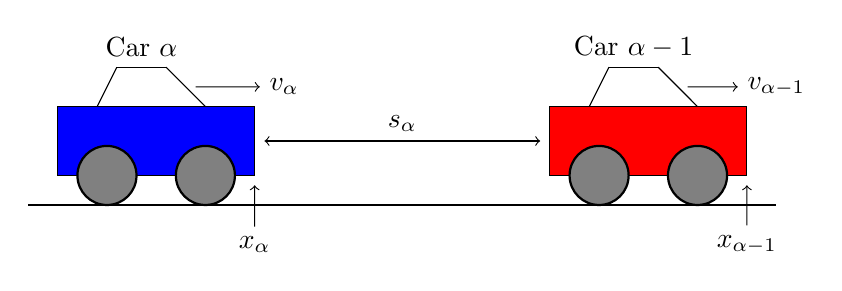
\begin{tikzpicture}[scale=1.25]
        \draw (-0.3,-0.3) -- (7.3,-0.3);
        \draw [fill = blue] (0,0) rectangle (2,0.7);
        \draw [fill=gray, thick] (0.5,0) circle [radius=0.3];
        \draw [fill=gray, thick] (1.5,0) circle [radius=0.3];
        \draw (1.5,0.7) -- (1.1,1.1);
        \draw (1.1,1.1) -- (0.6,1.1);
        \draw (0.6,1.1) -- (0.4,0.7);
        \node (car_a-1) at (0.85,1.3) {Car $\alpha$};
        \node (vel) at (2.3,0.9) {$v_{\alpha}$};
        \node (vel_start) at (1.3,0.9) {};
        \draw[->] (vel_start) -> (vel);
        \begin{scope}[shift={(5,0)}]
            \draw [fill = red] (0,0) rectangle (2,0.7);
            \draw [fill=gray, thick] (0.5,0) circle [radius=0.3];
            \draw [fill=gray, thick] (1.5,0) circle [radius=0.3];
            \draw (1.5,0.7) -- (1.1,1.1);
            \draw (1.1,1.1) -- (0.6,1.1);
            \draw (0.6,1.1) -- (0.4,0.7);
            \node (car_a-1) at (0.85,1.3) {Car $\alpha - 1$};
            \node (vel) at (2.3,0.9) {$v_{\alpha - 1}$};
            \node (vel_start) at (1.3,0.9) {};
            \draw[->] (vel_start) -> (vel);
          \end{scope}
        \node (x) at (2,0.35) {};
        \node (y) at (5,0.35) {};
        \node (x_pos) at (2,0) {};
        \node (x_sym) at (2,-0.7) {$x_{\alpha }$};
        \node (x_pos1) at (7,0) {};
        \node (x_sym1) at (7,-0.7) {$x_{\alpha - 1}$};
        \draw[<->] (x) -- node[above] {$s_{\alpha}$} (y);
        \draw[<-] (x_pos) -- (x_sym);
        \draw[<-] (x_pos1) -- (x_sym1);
        \end{tikzpicture} 
    \centering
    \caption{Defining index, position, velocity, and gap of a car.}
    \begin{itemize}
      \item $x_\alpha$, position of $\alpha$th car.
      \item $v_\alpha$, velocity of $\alpha$th car.
      \item $a_\alpha$, acceleration of $\alpha$th car.
      \item $s_\alpha$, gap of $\alpha$th car.
      \item Will denote the car $\alpha - 1$ by car $l$.
    \end{itemize}
\end{figure}  
\end{frame}

\begin{frame}
  \frametitle{Coupled Differential Equations}
  \begin{align*} 
    \odv{x_\alpha(t)}{t} &= v_\alpha (t), \\
    \odv{v_\alpha (t)}{t} &= a_{\rm mic} (s_\alpha, v_\alpha, v_l).
  \end{align*}
  Each car following model has a specific acceleration function: $a_{\rm mic} (s_\alpha, v_\alpha, v_l)$.
\end{frame}

\begin{frame}
  \frametitle{Full Velocity Difference Model}
  \begin{gather*}
      a_{\rm mic}(s_\alpha,v_\alpha,v_l) = \frac{v_{\rm opt} (s) - v_\alpha}{\tau} - \gamma \Delta v, \\
      v_{\rm opt} (s) = \max \left( 0, \min \left( v_0, \frac{s-s_0}{T} \right) \right).
  \end{gather*}
  \centerline{\rule{0.8\linewidth}{.2pt}}
  \begin{figure}[H]
    \begin{center}
      \begin{tabular}{c l c } 
      $v_0$ & desired speed  \\
      $s_0$ & minimum distance gap \\
      $T$ & time gap \\
      $\tau$ & speed adaptation time \\
      $\gamma$ & speed difference sensitivity \\
      \end{tabular}
      \end{center}
  \end{figure}
\end{frame}

\begin{frame}
  \frametitle{Graph of Optimal Velocity Function}
  \begin{figure}[H]
    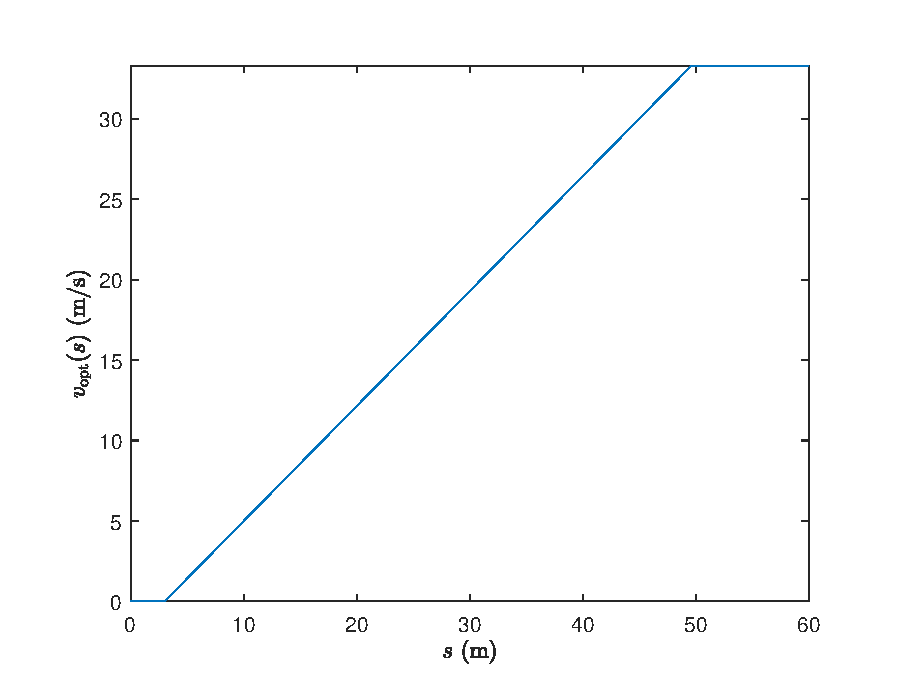
\includegraphics[width=9cm]{vopt_versus_s.eps}
    \centering
    \caption{Graph of the optimal velocity function over a range of gaps.}
\end{figure}
\end{frame}

\section{Implementation}
\begin{frame}
  \frametitle{Forward Euler Method Scheme}
  \begin{align*}
    v_\alpha(t+\Delta t) &= v_\alpha(t) +a_{\rm mic}(s_\alpha(t), v_\alpha (t), v_l (t))\Delta t, \\
    x_\alpha(t + \Delta t) &= x_\alpha(t) + \frac{v_\alpha (t) + v_\alpha (t+\Delta t)}{2}\Delta t.
\end{align*}
\end{frame}

\begin{frame}
  \frametitle{Pseudocode for FVDM}
  \begin{algorithm}
    \caption{Simplified algorithm for FDVM}
    \begin{algorithmic}
    \Require Initial state variables for each car at $t=0$. 
    \Require carArr, an array of cars.
    \For{$i = 1:$numsteps}{}
    \For{$j =$ length(carArr):$-1$:$1$}{}
      \State State variables of $j$th car $\gets$ Update $j$th car by a timestep.
      \EndFor
    \EndFor
    \end{algorithmic}
    \end{algorithm}
\end{frame}
\section{Examining Scenarios}

\subsection{Homogeneous Traffic}

\begin{frame}
  \frametitle{Homogeneous Traffic}
\end{frame}

\subsection{Obstacle}

\begin{frame}
  \frametitle{Obstacle}
\end{frame}

\subsection{Multi-lane Bottleneck}

\begin{frame}
  \frametitle{Multi-lane Bottleneck}
\end{frame}
\end{document}